\FloatBarrier
\subsection{HiST Optical Instrument}\label{sec:fushist}
The multi-site portable camera network know as phase 1 HiST \citep{hirsch2016} operates in a two camera mode with \unit[3.1]{km} separation between nodes as shown in Figure~\ref{fig:sitemap}.
\begin{figure}\centering
    \includegraphics[width=0.9\columnwidth,trim=0 400 0 0,clip]{gfx/3sites}
    \caption{Sites on the Poker Flat Research Range near Chatanika, Alaska used for analysis in this paper. PFISR: Poker Flat Incoherent Scatter Radar. HiST0/1: High-Speed Auroral Tomography camera sites.}
    \label{fig:sitemap}
\end{figure}
HiST cameras include the Andor iXon 897 and iXon 888, with notional parameters described in Table~\ref{tab:ixonrate}.
Auroral imaging systems spectral filtering choices include:
\begin{enumerate}
    \item white light (no filter inserted) \citep{donovan2006}
    \item narrow bandpass filter \citep{dahlgren2015}
    \item bandstop filter \citep{semeter2008,hirsch2016}.
\end{enumerate}
A comparison of bandstop filters typically used by prompt auroral imaging instruments is given in Figure~\ref{fig:filters}.
\begin{figure}\centering
    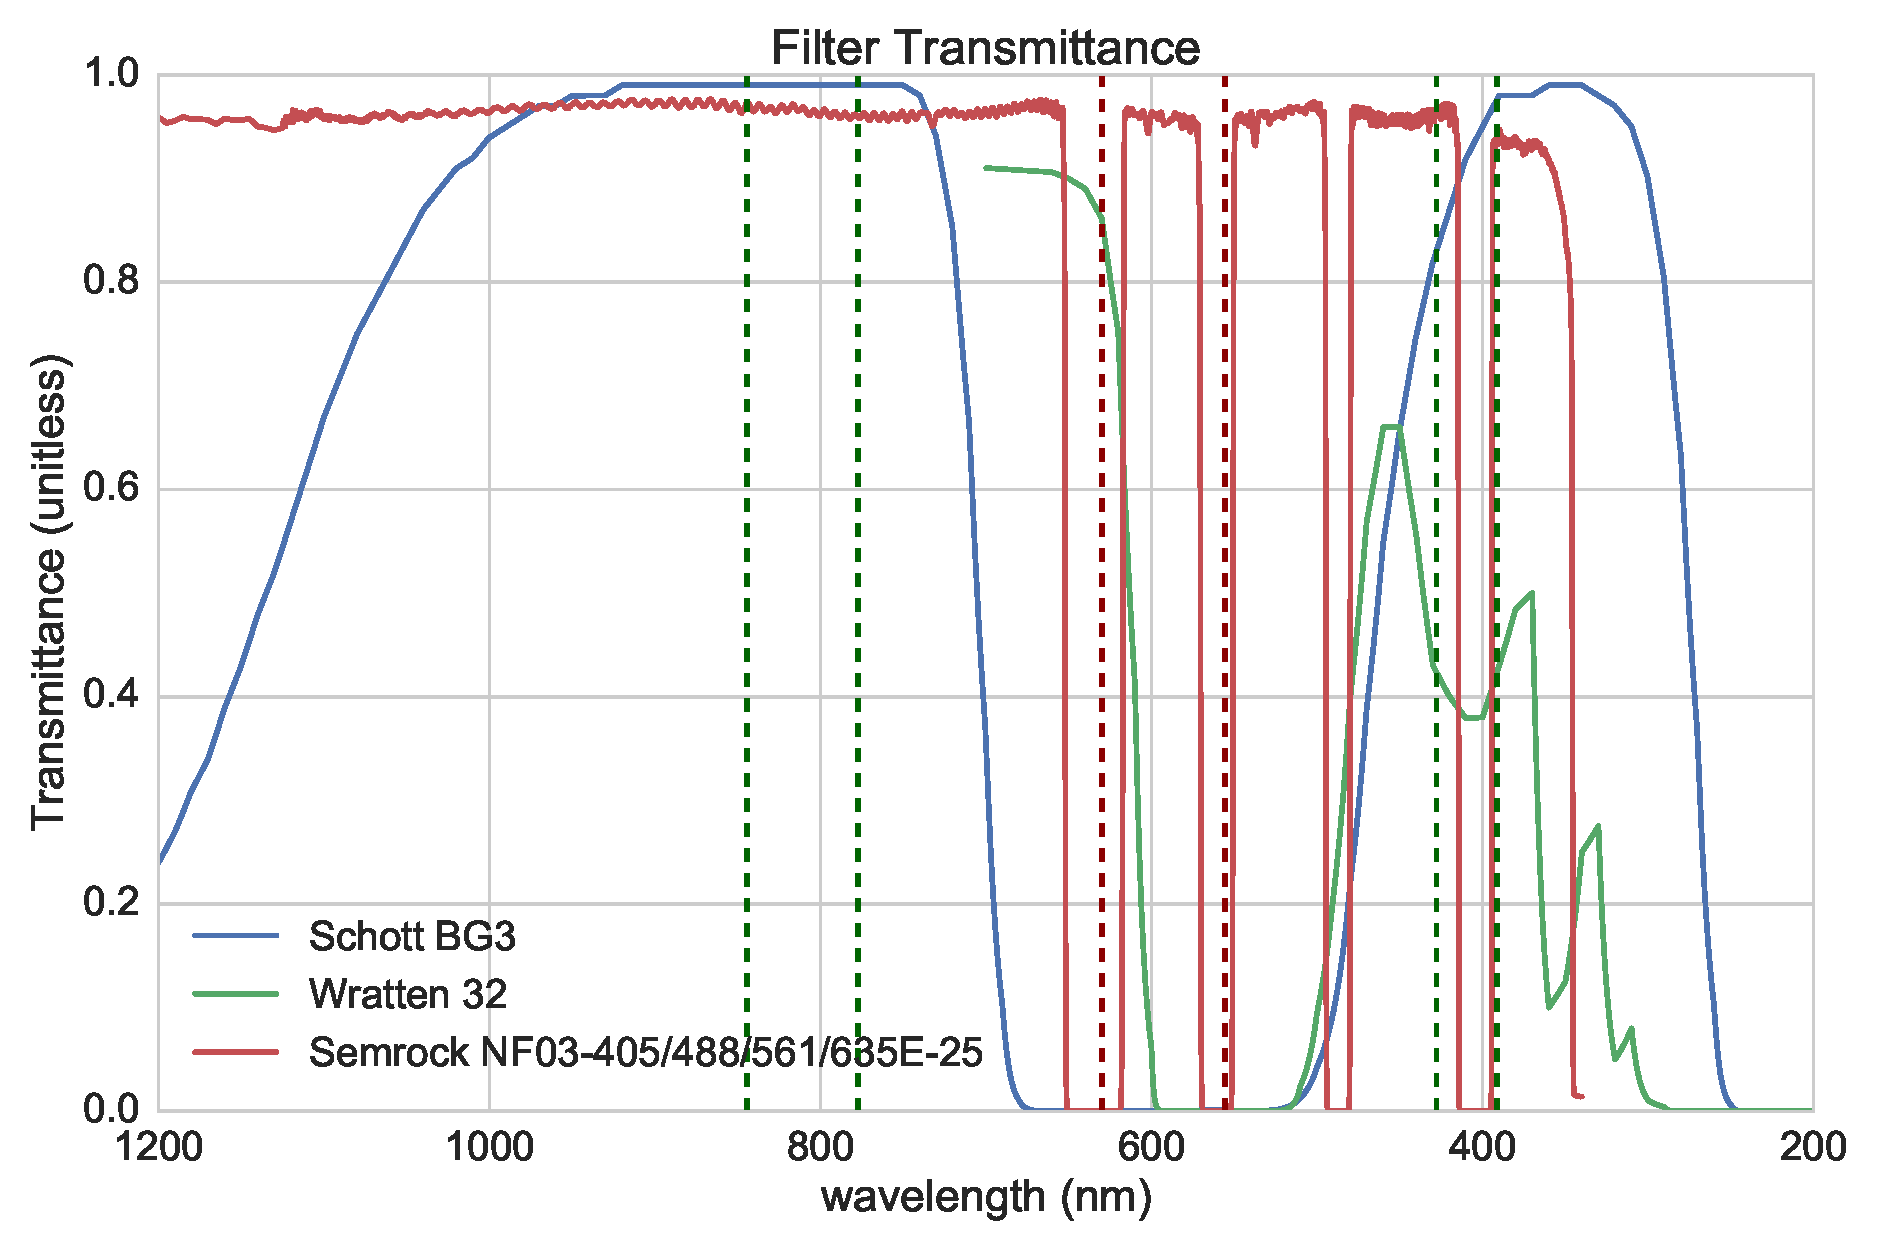
\includegraphics[width=0.9\columnwidth]{gfx/filterT}
    \caption{Comparison of bandstop filters used by other systems studying prompt auroral emissions with Schott BG3 bandstop filter used by HiST. Red markers at strong forbidden auroral emission wavelengths and green markers at strong permitted auroral emission wavelengths.}\label{fig:filters}
\end{figure}
The Wratten 32 filter \citep{wratten} has two deficiencies for fast auroral imaging: it passes the metastable oxygen emission at \unit[630]{nm} and has high attenuation of the NO emission at \unit[427.8]{nm}.
The Semrock NF03-405/488/561/635E-25 filter \citep{semrock} has similar performance \citep{jackel2014} for the auroral emissions of interest as the BG3 filters used for HiST.
HiST lenses yield a 9 degree field of view approximately centered on magnetic zenith, similar to the MOOSE instrument but HiST has significantly higher spatial resolution.
Star registration is via the astrometry.net software \citep{lang2010,hirschastro}, allowing a common local coördinate system to be created for PFISR and HiST \citep{geodata}.

The first considerations for designing a prompt auroral emissions observatory, whether based on ground, rocket or satellite include:
\begin{enumerate}
    \item Optical filtering: white light or no filtering will cover over prompt emissions with stronger, smeared forbidden emissions such as $\lambda = \unit[557.7]{nm}$, the first measured auroral emission line \citep{angstrom1869}.
    Shortpass filtering such as used in \citet{nishiyama2016} discards the medium brightness N$_2$ 1P \unit[670]{nm} and OI $\in \{777.4, 844.6\}$~nm emissions.
    Narrow-bandpass filtering discards most of the physical processes, leaving only part of the particle energy deposition picture available for estimation.
    HiST takes the bandstop filter approach, retaining most of the prompt emissions while discarding most forbidden emissions.
    \item Data inversion: remote observatories must either transmit or store data suitable for physical quantity estimation. HiST uses a unique implementation of model based iterative reconstruction (MBIR).
    MBIR reduces the dimensionality of difficult tomographic problems, thereby requiring less SNR for a given error level.
    In the medical field, MBIR is credited with reducing patient CT radiation doses by up to 98\% \citep{liu2014}.
    \item Data curation: MBIR estimation is known for being modestly time-consuming to compute.
    Currently, a single \unit[20]{ms} HiST frame takes about one minute to reconstruct a $\Phi_{top}(E,x)$ estimate \citep{hirsch2016}.
    To conserve human and computing resources, an on-site automatic data curation algorithm \citep{cviono} was developed and implemented \citep{hirsch2016bigdata}, allowing indefinite operating lifetime with yearly external USB 3.0 hard drive swap.
\end{enumerate}

Electron precipitation along $B_\parallel$ may be described by particle penetration models yielding wavelength-dependent optical intensity.
Auroral lines relevant to the filter selection of Figure~\ref{fig:filters} are listed in Table~\ref{tab:spectrum}.
\begin{table}\centering
    \caption{Selected auroral emission lines}\label{tab:spectrum}
    \begin{tabular}{rllll}
        \toprule
        $\lambda$ [nm] & family  & HiST system loss [dB] & lifetime [sec.] \\
        \midrule
        %297.2 &  [OI]31     & 13.5 & \\ % not visible due to O3 absorption (Chamberlain ch 5.1 p. 185)
        337.0 & N$_2^+$ 2P (0,0) &      &  \\
        % ~339.5 & N2+ 2P(3,6) \\
        391.4 & N$_2^+$ 1N (0,0) & 2.0  & $70 \times 10^{-9}$ \\ % high energy precip, V. Jones, 1971
        % ~394.3 & N2+ 2P(2,5) \\
        427.8 & N$_2^+$ 1N (0,1) & 1.7  & \\ % 25 R/nm
        470.9 & N$_2^+$ 1N & & \\
        486.1 & H$_\beta$ & & \\ % weak proton aurora 50-300R
        519.8, 520.0 & [NI]21 & & 1 day \\ % may be as strong as 557.7 forbidden (Chamberlain p.186)
        557.7 & [OI]32  (1s) & 28.9 & 0.74 \\ % 1190 R/nm  forbidden
        % 587.6 & He (3P-3D) & & \\ % rarely (P.E. Sandholt, Dayside and Polar Cap Aurora)
        % 589.0/589.6 & Na (2S-2P) & & \\ % occasionally (P.E. Sandholt, Dayside and Polar Cap Aurora)
        630.0 & [OI]21      & 49.7 & 107 \\  % 810R/nm forbidden
%        656.3 & H$_\alpha$ & & \\ % weak proton aurora 50-300R
        670.0 & N$_2$ 1P & &  \\ % prompt, NOT N2+
%        732.0,733.0 &    [OII] $^2$P-$^2$D & & \\ % 100eV, high altitude.  Sullivan et al
        750.0 & N$_2$ 1P & &  \\ % prompt, NOT N2+
        %761.9 &   &    & 0.9 \\ %not ground-visible: 02 absorption (Vallance Jones 1974)
        777.4 & OI   3s-3p  & 1.1 & \\  % low energy precip, quintet (chamberlain p.188) permitted
        844.6 & OI   3s-3p  & 2.3 & \\  % low energy precip, triplet permitted
        \bottomrule
    \end{tabular}
\end{table}
The temporal behavior along $B_\parallel$ help reveal the mechanism driving a particular auroral morphology.
\citet{hirsch2016} showed that using two or more tightly-synchronized high-speed cameras separated by \unit[1..10]{km} and co-aimed at magnetic zenith has high spatio-temporal resolution without the inherent ambiguities of \textit{a priori} starting altitude made necessary in single-camera studies.
Thus, DAW and inverted-V aurora for discrete arcs, even closely $B_\perp$-spaced arcs can be distinguished with HiST.

Based on rocket measurement and theory, fine spatio-temporal $B_\perp$ auroral structure comes from DAW.
HiST analysis uses a physics-based ionospheric forward model for electron precipitation in the \unit[50]{eV}..\unit[18]{keV} range with two high-speed cameras spaced \unit[3]{km} apart.
Model-based iterative reconstruction is used to estimate the differential number flux of the particles versus space and time at the top of the ionosphere.
We define the top of the ionosphere as the region below which particle acceleration is neglected and above which energy deposition is neglected.
In this manner, tightly time-synchronized camera data at \unit[30]{ms} cadence combined with ISR measurements at \unit[100]{ms} cadence yield confirming evidence for the association of DAW with strong turbulence in the lower ionosphere.

The phase 1 HiST \unit[30]{ms} observational cadence is fast enough \citep{peticolas2000,hirsch2016} to observe signatures of DAW-accelerated particle precipitating into the ionosphere.
As implied by the name, dispersive acceleration leads to higher energy particles arriving at the ionosphere first, and therefore depositing their energy in the E-region ionosphere before the lower energy particles of the same magnetospheric particle batch arrive.
The time delay between high and low energy particles is only a few hundred milliseconds \citep{dahlgren2013}, so the HiST sampling cadence gives several estimates of auroral precipitation characteristics during a dispersive impulse, sufficient to resolve key parameters of the event such as characteristic energy and beam location versus time \citep{histfeas}.
